\subsection{Previous and Related Works}
These are projects that accomplished similar objectives to what we hope to accomplish or highlight a technology we plan to work with.
\subsubsection{DIY near-IR spectrometer}
Yuan Cao is a Ph.D. student at MIT with a blog where he posts his unofficial projects. He published a project titled “A \textdollar500 DIY near-IR spectrometer that would sell for \textdollar10,000.” In it, he describes his idea, designs and results for a low cost infrared spectrometer. His design features surprisingly high performance for its price. The system uses an InGaAs photodiode, a reflective diffraction grating, a fiber collimator, some cheap optics, and a microcontroller to create a spectrograph of any light source. It boasts very high signal to noise ratios, 5-6nm spectral resolution, and a price point under \textdollar500. There are definitely some design features worth imitating, specifically the diffraction grating “scanner” that is rotated to pass wavelengths across the surface of the photodiode, as well as the filter circuitry that cleans up the electrical signal. 
\begin{figure}[H]
    \caption{Yuan Cao DIY NIR Spectrometer}
    \centering
    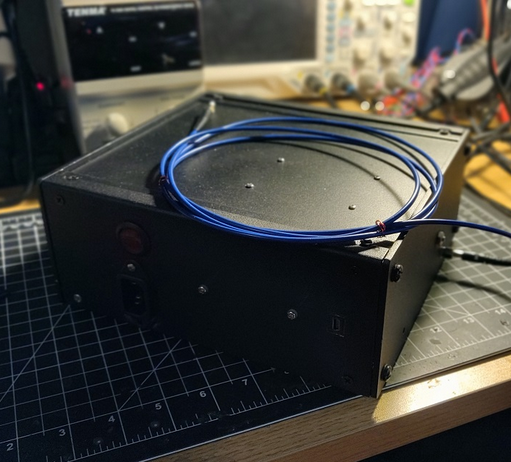
\includegraphics[width=0.5\textwidth]{images/3-1-1Pic.png}
\end{figure}
That said, there are some reasons why this project differs in application from the Auto Garden Bed Near Infrared Spectrometer. First, the detector has a spectral range from 800 – 1600nm. This is the Near Infrared Regime, but it is not very far into the NIR, which in some contexts refers to wavelengths as far out as 2500nm. If Soil Spectroscopy requires this depth, or frequencies in the visible spectrum, the design will have to be modified. Second, this system was built for lab use, specifically to characterize light sources. The reported data was very promising, but in every case the spectrometer targeted an object that was emitting strong optical power in every direction. Soil does not fluoresce, so the Auto Garden Bed will require additional components to probe the soil with an electromagnetic wave. In the end, what’s most important is that this project demonstrates that low cost spectroscopy can be achieved.


\subsubsection{Chlorophyll Flourescence Spectrometer}



In 2021 UCF’s ECE Senior Design Group 1 designed a Chlorophyll Fluorescence Spectrometer. The purpose of this project was to design a system that would detect chlorophyll in plants through stimulation by UV rays. It featured a diffraction grating and a monochromatic CMOS sensor. It is interesting to note that unlike the previously explored project, spatial separation of light frequencies is achieved with a monochromatic camera. This means that each intensity can be mapped to the position on the cmos sensor, and the system can “stare” rather than “scan.” Eliminating moving parts is a major benefit in projects requiring sensitive optical alignment, making this a feature worth seriously considering.

\begin{figure}[H]
    \caption{Chlorophyll Flourescence Spectrometer}
    \centering
    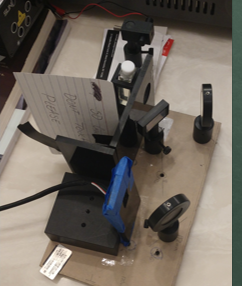
\includegraphics[width=.5\textwidth]{images/3-1-2Pic.png}
\end{figure}

This project produces a design with similar goals to the Auto Garden Bed, because it features a light source, a target object, focusing optics, wavelength selection, and generating and interpreting a spectrograph. However, the optical regime of UV rays may be limited to fluorescence spectroscopy and unfit for proximity soil sensing. The research will have to determine what sensors are viable and whether this imposes further constraints on the system.

\subsubsection{Smart Garden Controller}
The Smart Garden Controller was a UCF senior design project with very similar motivations to the Auto Garden Bed. The goal was to create a system that reduced user labor by automating the irrigation schedule of garden areas and reducing waste by sensing moisture levels\cite{smart-garden-controller}. The system was also designed to anticipate the informational needs of the gardener and come prepared with a set of popular vegetables and plants, corresponding to variables the team had already investigated to maximize flourishing. It used sensors to detect the health of the plant environment, a microcontroller to facilitate irrigation, and a web API to interface to the user for control of the system. The group also set goals to offer ease of setup, competitive price, and Smart Device integration by integrating with a device like Amazon’s “Alexa.” The last similar design features are wall plug power consumption, lithium ion battery backup power, and http secure information protocol over wifi.
\begin{figure}[H]
    \caption{Smart Garden Controller}
    \centering
    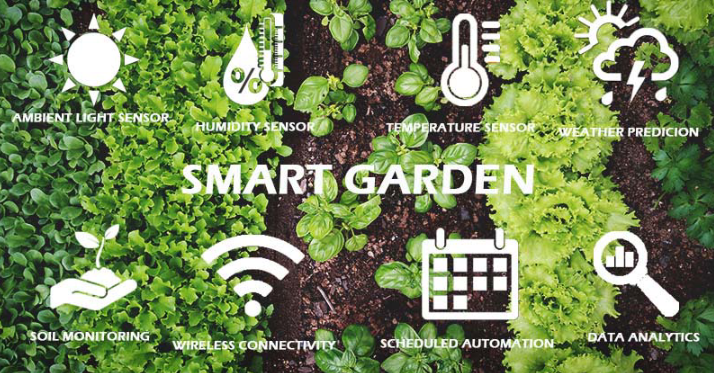
\includegraphics[width=0.5\textwidth]{images/3-1-3Pic.png}
\end{figure}
This project features much of the same core functionality as the Auto Garden bed, however, closer review of the scope and feature set reveal that the designs are incompatible. The Smart Garden Controller was designed to facilitate more precise control of an entire garden, allowing the user to isolate different areas for growing different plants. The area of interest was 100 squared feet, and the system was intended to relieve the gardener of the complication of watering each section for different amounts of time. This meant a wide reaching irrigation network as well as a network of sensors throughout the yard. The scope of the Auto Garden Bed allows for single source irrigation and sensing, which allows for greater flexibility of mechanical design, including power generation and environmental controls.

\subsubsection{Automated Rotating Solar Plant Rack with Self-care Capabilities}

This is another home garden system with a different target solution. The goal is to facilitate the growth of indoor plants and ensure maximum plant health by rotating the plant base so that the forces driving it to grow sideways cancel out in every direction. Like previous projects, the system is integrated with wireless communication and a schedule selector for different plant types. Unlike previous projects, one of the means of achieving plant health is by protecting sensitive plants from excessive exposure to sunlight, which is a feature that the Auto Garden Bed seeks to implement. 

\begin{figure}[H]
    \caption{Automated Rotating Solar Plant Rack}
    \centering
    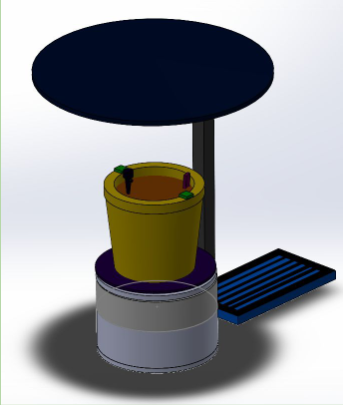
\includegraphics[width=.5\textwidth]{images/3-1-4Pic.png}
\end{figure}

Another point of interest in the Automated Rotating Solar Plant Rack is its rotating foundation. Maximizing sun exposure is a goal of this project, and although the application is energy collection, there may be parallel design opportunities with the Solar Plant Rack.


\subsubsection{Stem 'n' Leaf}
Stem 'n' Leaf is a UCF Senior Design project. The focus of this project was to be a ``modular hydroponics system'' wherein each plant unit can be fed my a singular control unit. Thus, the ``stem'' is the control unit and the ``leaves'' are the plant units\cite{stem-n-leaf}. Their design was focused on modularity and scalability. Hence their design is stackable and tileable design of the bed itself. The key features of this plant bed is that it self-regulates pH and integrates with a mobile application.
\begin{figure}[H]
    \caption{Stem 'n' Leaf}
    \centering
    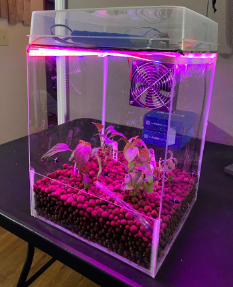
\includegraphics[width=.5\textwidth]{images/3-1-5Pic.png}
\end{figure}

The project uses a liquid pH-sensor to obtain the relevant data. Our team wants a similar result but will be trying to achieve this via optical means. Their team mentioned the durability of the sensor which is our team's chief concern seeing as acidic and basic solutions tend to be corrosive and promote oxidation of metals thus the optical approach should improve longevity of the project. 

\subsubsection{Green Steel Garden}
Green Steel Garden is another UCF Senior Project that our team is pulling some inspiration from. Another hydroponics system that measures soil nutrients and pH for controlling the parameters of the garden bed\cite{green-steel}. The key feature of this project is the nutrients system and the pH sensor.

\begin{figure}[H]
    \caption{Green Steel Garden}
    \centering
    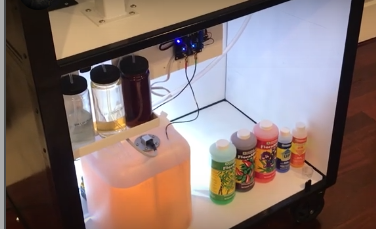
\includegraphics[width=0.5\textwidth]{images/3-1-6Pic.png}
\end{figure}

This project utilizes a water reservoir and reservoirs of chemicals to balance the pH of the water entering the garden bed. They use peristaltic pumps to accomplish the mixture and a combination of pH and electrical conductivity sensors to get data from the water. The current design consensus for our team is that we will be hooked up to hose which is limited by a solenoid valve, but being able to ``treat'' the water that is entering the system may be a design decision that has to be considered.

\subsubsection{Summary}

The previous works discussed here highlight the key components of our garden bed: sensing in conjunction with optics. Something of note in these deliberations is the use of hydroponics in all of these projects; something that is rendered unnecessary and seemingly inefficient in an outdoor garden bed.

The previous works related to optics focus on wavelengths outside of our team's consideration (Infrared), instead focusing on UV and visible light through near-Infrared. Their research highlighted potential flaws in some assumptions we had made. Firstly, that it is possible to reduce the moving components of our optical sensing, obtaining a wider field. Secondly, that using IR spectroscopy is practical for getting data from soil as it is used in commercial projects today and shows tremendous value in commercial sectors.

Most of the other garden bed projects focus on hydroponics but something of interesting note is the rotating solar rack project. The control scheme regarding the degrees of rotational freedom and the means of achieving success will be paramount in implementing our own moving solar array. Of interesting note is that all the other garden bed projects focused primarily on hydroponics as it gives greater measures of control to the soil nutrients which had not been a consideration of our team before looking into the previous works. Instituting a chemical pump into our design may be necessary to achieve our goal of being ``set it and forget it'' while still providing updates for when to refill the chemical tanks of integration with the water.

All of the garden projects tried to integrate some means of a mobile app or web user interface. They all mentioned that they needed to have started this component earlier. Each of the mobile application projects were not able to achieve this by their final meeting which is of special concern. Also of note is their choice of stack; many of the projects chose a NoSQL stack which seems counterintuitive given the highly relational nature of the data that is being collected. Our team can learn from this by starting this integration as early as possible and choosing to implement the smallest possible feature set that accomplishes the goals.
